%! Author = johannes
%! Date = 03.01.23

\subsection{JNDI}\label{subsec:jndi}
\begin{wrapfigure}{r}{0.5\textwidth}
    \begin{center}
        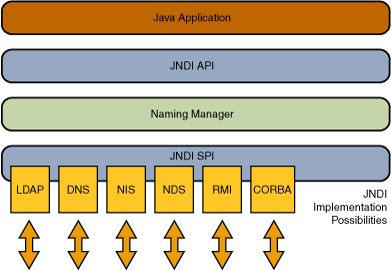
\includegraphics[width=0.48\textwidth]{images/jndiarch}
    \end{center}
    \source{\href{https://docs.oracle.com/javase/tutorial/jndi/overview/index.html}{Oracle Docs}}
    \caption{JNDI Architektur}
\end{wrapfigure}
Das \gls{jndi} ist ein \gls{spi} und bereits seit den 90ern\footfullcite{jndiHackTricks} Teil der Java SE.
\glsaccessshort{jndi} wird zur Verbindung mit externen Java Ressourcen wie beispielsweise Datenbanken verwendet.
Da \glsaccessshort{jndi} modular aufgebaut ist, existieren mehrere Interfaces um verschiedene Namens- oder Verzeichnisdienste zu verwenden.
Die am häufigsten verwendeten Dienste sind dabei \gls{ldap}, \gls{rmi}, \gls{dns} und \gls{corba}.
